\chapter{Deep Learning for 21cm Observations}
\label{chapter:hera_ml}

Modern cosmological theory is capable of predicting the statistical features of many aspects of the observable Universe, using either theoretical calculations \citep[e.g.][]{Bond.91, Sheth.99} or sophisticated numerical simulations \citep[e.g.][]{Lewis.00, Vogelsberger.14}. These theories may be tested by making observations of various large-scale fields, in surveys spanning large cosmological volumes in space and time. The ultimate goal of measurements is extract from the data some parameters which are believed to describe the underlying processes, and to relate these parameters to a theoretical understanding of the physics at work. In some cases -- most conspicuously the primordial CMB -- the statistics of the fields are Gaussian, and are completely described by the two-point correlation function, or its Fourier conjugate, the power spectrum \citep[e.g.][for a review]{Liddle.00}.

A field described only by Gaussian statistics practically does not exist in cosmology beyond the CMB. For nearly every other scenario involving the non-linear interactions of gravity, radiation, and fluid mechanics, the resultant fields are non-Gaussian. Within the non-Gaussianity of these fields is encoded additional valuable information about the astrophysical processes at work, and can also serve as a cross-validation of two-point statistics of the same field \citep{Alvarez.16, Majumdar.17}. The specific details of the non-Gaussianity are not usually straightforwardly obtained from the theory, and thus devising appropriate higher-order statistics to efficiently probe the non-Gaussian information is in general a difficult problem. 

By analyzing a field using power spectra, one explicitly neglects all non-Gaussian information. In Chapter~\ref{chapter:ksz_21cm}, we presented higher-order correlation functions that are sensitive to non-Gaussian information in Fourier space. In the case of 21\,cm emission, working in Fourier space provides a natural and relatively simple way to avoid foreground contamination. Another solution could be to search for non-Gaussian information in image space, assuming some future development that could overcome the foreground challenge \citep[e.g.][]{Shaw.14, Shaw.15, Zhu.16, Patil.17}, or that we may operate on wedge-filtered image fields in a physically meaningful way \citep{Beardsley.15}. Staying in image space allows us to retain the non-Gaussian information in our data.

\section{Neural Networks}

A potential solution for parameter extraction is available due to advances in computation, allowing us to generate large numbers of numerical simulations which are realizations that capture the relevant physics of an astrophysical process \citep[e.g.][]{Mesinger.11}, and the development of deep learning algorithms which can be ``trained" to recognize patterns in data \citep[e.g.][]{Hinton.06, Hinton.12}.

Convolutional Neural Networks \citep[CNNs; e.g.][]{Lecun.95} have proven exceptionally useful for extracting non-Gaussian information from images in order to classify or extract information from their contents to a very high accuracy \citep[e.g.][]{imagenet.12}. There are many, many explanations of the inner calculus of neural networks, and the intention of this chapter is not a comprehensive review of that field. For the purposes of this chapter, a few concepts must be mentioned:

\begin{itemize}
\item Convolutional Neural Networks are systems of 1, 2 or 3-dimensional matrices that are used as convolutional kernels on an input image. An image is propagated forward through the network via consecutive convolutions by these kernels. Each kernel entry (i.e. pixel) is known as a `weight' $w$.

\item The desired output of a `training set', for example, the contents of an image, is given as a vector which the total of all the convolutions must reproduce.

\item Inevitably, if the convolutional kernels are initially randomly generated, the output vector will not contain the desired quantities. A `cost function' is a metric that specifies how `wrong' an output is. This could be the mean squared error, for example.

\item Neural networks `learn' through a process called `backpropagation'. Based on the cost function, a chain rule can be applied backwards along the network for each input, updating the values of the weights by some fraction of the user-specified `learning rate' \citep{Rumelhart.86}.

\item Associated with each weight is an `activation function', $a(x)$. The value of $a(w*x)$ (the output of the activation function given the convolved input) is actually what is handed to the next convolutional kernel along the network. Activation functions can be non-linear, allowing neural networks to learn complex decision boundaries.

\item In order to down-sample the data to a more manageable size, `pooling layers' are often implemented. These extract a moving statistic such as the moving average or maximum in a given region of the image.

\item CNNs often end with a `fully connected' or `dense' layer. These are multi-layer perceptrons \citep[e.g.][]{Rosenblatt.61} that propagate the value s of $a(wx)$ -- that is, no convolution is applied, and each layer is 1-dimensional.

\item After training on some subset of the total data (which may be done several times over), a neural network can be `tested' by forward-propagating new images, not used in training, and not backpropapating. Testing can also be implemented after some subsample of the training data has been propagated -- i.e., as the network is in the middle of training -- often called `validation'.
\end{itemize}

With this primer in mind, we will present two uses of CNNs for understanding simulated realizations of reionization: classifying the main causes (galaxies or active galactic nuclei) of reionization \citep{Sultan.18}, and regressing upon a physical parameter of interest.

\section{Reionization model classifier}

The 21\,cm power spectrum is a powerful tool for quantifying the relative clustering of large and small scaled ionized regions \citep{Hassan.17}. However, the topology of the regions themselves can provide information on the dominant mechanism of their formation. We considered two scenarios: one in which only galaxies, and the other in which only active galactic nuclei (AGN), provided ionizing photons. 

We used {\sc simfast21} \citep{Santos.10, Hassan.17.1} to generate a dark matter density field, evolve it into the non-linear regime using the Zel'dovich approximation. Dark matter halos were generated using the excursion set formalism \citep{Bond.91}. Either galaxies or AGN were placed in halos, with populations following the parametrization of \cite{Hassan.16}. Ionized regions are ``painted on top of" the dark matter halos according to parametrizations from high-resolution radiative transfer simulations and large-volume hydrodynamic simulations (see \cite{Hassan.16, Hassan.18}). An example of a galaxy-dominated and AGN-dominated reionization field is shown in Figure~\ref{fig:hassan-fields}. For this study, we focused on the field at redshift $z=8$. Galaxies produce more, small, ionized regions, whereas AGN produce larger more spherical ones. This is due to the strong clustering AGN and their harder X-ray spectrum.

\begin{figure}
\centering
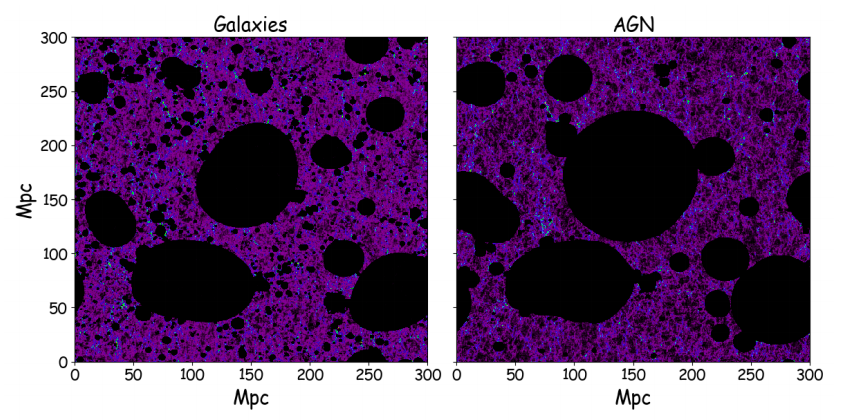
\includegraphics[width=0.8\textwidth]{chapters/hera_ml/figures/hassan-field.png}
\caption[21\,cm brightness temperature fields for Galaxy-Only and AGN-only models.]{21\,cm brightness temperature fields (in arbitrary units) for Galaxy-Only (left) and AGN-only (right) models. Figure from \cite{Hassan.18}.}
\label{fig:hassan-fields}
\end{figure}

We used {\tt Tensorflow} to build a classifying CNN with 2 layers of 2-dimensional convolutional kernels interleaved with two maximum-pooling layers, a single dense layer, and an output layer. The convolutional and dense layers used the ReLU activation function, which is defined as

\begin{equation}
{\rm ReLU}(x) = 
\begin{cases} 
      0 & x < 0 \\
      x & x >0 
\end{cases}
\end{equation}

\begin{figure}
\centering
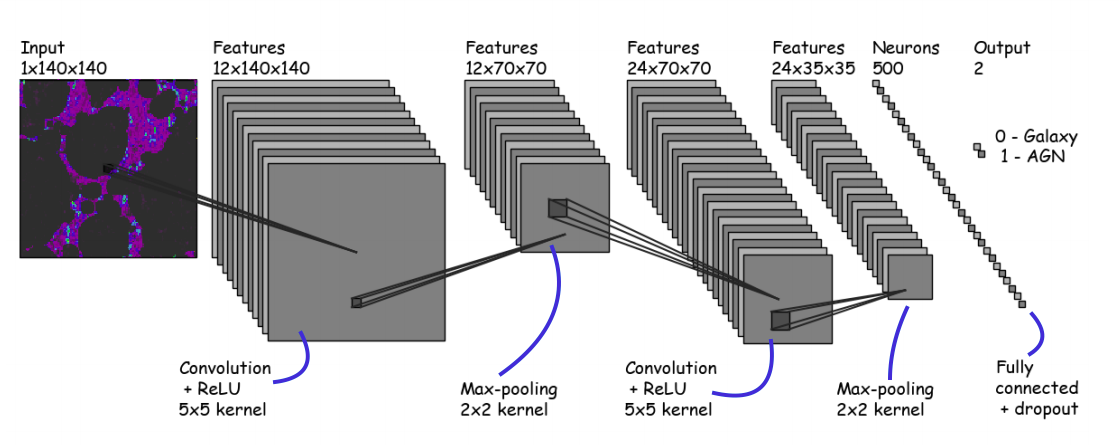
\includegraphics[width=0.8\textwidth]{chapters/hera_ml/figures/hassan-cnn.png}
\caption{The classification CNN used in this study.}
\label{fig:hassan-cnn}
\end{figure}

The network is shown in Figure~\ref{fig:hassan-cnn}. To train it, we used $\sim 1000$ images of $z=8$ realizations. Each image was a $140\times140$ greyscale image of 21\,cm brightness temperature, with a simulation box size of 75\,Mpc. Each image came from a separate simulation, which varied the photon escape fraction, X-ray spectrum of the ionizing sources and the ionizing efficiency of those sources. The testing set was $\sim 100$ additional images. To prevent over-fitting, only a random set of 75\% of neurons were used during each forward propagation (known as `dropout').

Using the {\sc 21cmSense} package \citep{Pober.14}, we could simulate the expected thermal noise of a foreground-decontaminated image cube for LOFAR, HERA-331 and SKA-Low (see Chapter~\ref{chapter:instruments}). Adding this noise to each image allowed us to make predictions of the accuracy of such a tool for predicting ionization models for actual data.

The results of training and validation are shown in Figure

\section{Reionization parameter regressor}

\section{Future directions}
This is an effort ripe for exploration...
%
% - understanding kernels
% - extraction of the bispectrum
% - cross-correlation with multiple inputs
% - visibility data (harken back to data processing chapter)